\documentclass[]{report}
\usepackage{graphicx}
\usepackage[a4paper,left=1.5in,right=1in,top=1in,bottom=1in]{geometry}
\fontsize{14}{16}\selectfont
\author{Krishna Acharya}
\begin{document}
\begin{titlepage}
    \noindent
    \begin{center}
        
\includegraphics[width=4cm]{img/logo.png}

        {\fontsize{12}{14.4} \bfseries \centering TRIBHUVAN UNIVERSITY \\ INSTITUTE OF ENGINEERING \\ THAPATHALI CAMPUS \\ }

        \vspace{1.5cm}

        {\bfseries A Lab Report of Microprocessor \\ LAB -3 \\ Logical Instruction Set \linebreak[4] \\}

        \vspace{0.75cm}

        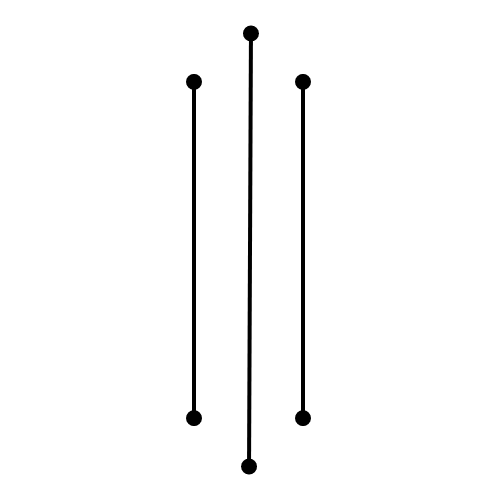
\includegraphics[width=7cm]{img/vline.png}

        \vspace{0.75cm}

        {\bfseries Submitted By:} \\

        Name: Krishna Acharya \\
        Roll No.: THA078BEI010 \\

        \vspace{1cm}

        {\bfseries Submitted To:} \\
        Department of Electronics and Computer Engineering \\
        Thapathali Campus \\
        Kathmandu, Nepal \linebreak[5] \\
        \today \\
    \end{center}

\end{titlepage}

\section*{OBJECTIVES}
\begin{itemize}
 \item  To Gain Proficiency in the 8085's Logical Instruction Set through Experimental Learning
\end{itemize}

\section*{EQUIPMENTS REQUIRED}
\begin{itemize}
 \item 8085 learning kit
 \item Simulator for 8085 microprocessor
\end{itemize}

\section*{THEORY}
A microprocessor is a basically a programmable logic chip. It can perform all the functions of the hard-wired logic through its instruction set. The 8085 instruction sets includes such logic functions are as follows: \\



% \begin{tabular}{lll}
\begin{tabular}{p{2cm} p{2cm} p{9cm}}
    \hline
    Mnemonics & Examples & Operation \\
    \hline
    ANA R & ANA B & Logically AND the contents of a register with A \\
    ANI 8-bit & ANI 2FH & Logically AND the 8-bit data with A \\
    ANA M & ANA M & Logically AND the contents of M with A \\
    ORA R & ORA E & Logically OR the contents of reg E with A \\
    ORI 8-bit & ORI 3FH & Logically OR the 8-bit data with A \\
    ORA M & ORA M & Logically OR the contents of M with A \\
    XRA R & XRA B & Logically XOR the contents of B with A \\
    XRI 8-bit & XRI 6AH & Logically XOR 8-bit data with A \\
    XRA M & XRA M & Logically XOR the contents of M with A \\
    CMP R & CMP B & Compare the contents of register with the contents of A for less than , greater than or equal to \\
    CPI 8-bit & CPI 45H & Compare the 8-bit data with the contents of A for less than, greater than or equal to \\
    RLC & RLC & Rotate accumulator left i.e. \emph{Each bit is shifted to adjcent left positions. Bit D7 becomes Do} \\
    RAL & RAL & Rotate accumulator left through carry \emph{Each bit is shifted to the adjcent left position. Bit D7 becomes the carry bit and the carry bit is shifted to Do.} \\
    RRC & RRC & Rotate accumulator right \emph{Each bit is shifted right to the adjcent position and Bit Do becomes D7} \\
    RAR & RAR & Rotate Accumulator Right through carry \emph{Each bit is shifted right to the adjcent position. Bit D7 becomes carry bit and the carry bit is shifted into D7} \\
    CMC & & Complements the carry flag. \\
    STC & & Sets the carry flag \\
    CMA & & Complements the accumulator. \\

    \hline
\end{tabular}
\vspace{5mm}
\\
The following features hold true for all the instructions:
\begin{enumerate}
\item The instructions implicitly assume accumulator as one of the operand
\item All instructions reset carry flag except for the complement where carry flag remains unchanged
\item They modify Z, P and S flags according to the data conditions of the result
\item Place the result in the accumulator
\item They do not effect the content of the operand register
\end{enumerate}

\section*{INITIAL PART}
\subsection*{Example 1:}
Load the following Program and check the output of flags
\subsubsection{Code}
\begin{verbatim}
    MVI A, 82H
    MVI B, 52H
    ANA B
    ANI 45
    RST 5
\end{verbatim}
\subsubsection{Flags}
\begin{tabular}{cccccccc}
\hline
    S & Z & *  & AC & *  & P & *  & CY  \\
    \hline
    0&1&0&1&0&1&0&0\\
    \hline
\end{tabular}
\subsubsection {Register Table}
\begin{tabular}{lc}
    \hline
    Register & Value\\
    \hline
    Accumulator     & 00        \\
    Register B      &  52        \\
    Register C      &  00        \\
    Register D      &   00       \\
    Register E      &   00       \\
    Register H      &  00        \\
    Register L      &  00         \\
    Memory(M)       &      3F         \\
    \hline
\end{tabular}
% \subsubsection {Memory Table}
% \begin{tabular}{lc}
%     \hline
%     Memory Address & Value  \\
%     \hline
%     Memory(M)       &      3E         \\
%     \hline
% \end{tabular}
% \subsubsection {I/O Port Table}
% \begin{tabular}{lc}
%     \hline
%     Address & Value  \\
%     \hline
%     Memory(M)       &      3E         \\
%     \hline
% \end{tabular}

\vspace{10mm}
% example 2
\subsection*{Example 2:}
Load the following program and check the content of the respected registers and flag contents before and after XRA and ORA operations. Check out the XRI and ORI operations yourself.
\subsubsection{Code}
\begin{verbatim}
    MVI A, 8F
    MVI C, A2
    ORA C
    MVI D, 74
    XRA D
    RST 5
\end{verbatim}
\subsubsection{Flags}
\begin{tabular}{cccccccc}
\hline
    S & Z & *  & AC & *  & P & *  & CY  \\
    \hline
    1&0&0&0&0&1&0&0\\
    \hline
\end{tabular}
\subsubsection {Register Table}
\begin{tabular}{lc}
    \hline
    Register & Value\\
    \hline
    Accumulator     & DB            \\
    Register B      &  00        \\
    Register C      &  A2        \\
    Register D      &   74       \\
    Register E      &   00       \\
    Register H      &  00        \\
    Register L      &  A2         \\
    Memory(M)       &      00         \\
    \hline
\end{tabular}
% \subsubsection {Memory Table}
% \begin{tabular}{lc}
%     \hline
%     Memory Address & Value  \\
%     \hline
%     Memory(M)       &      3E         \\
%     \hline
% \end{tabular}
% \subsubsection {I/O Port Table}
% \begin{tabular}{lc}
%     \hline
%     Address & Value  \\
%     \hline
%     Memory(M)       &      3E         \\
%     \hline
% \end{tabular}






\vspace{10mm}
% example 3
\subsection*{Example 3:}
Load the following program and check out the flag contents to find which number is greater.
\subsubsection{Code}
\begin{verbatim}
    MVI A, 72H
    LXI H, 8010
    CMP M
    CMP H
    CPI 72H
    RST 5
\end{verbatim}
\subsubsection{Flags}
at CMP M \\
\begin{tabular}{cccccccc}
\hline
    S & Z & *  & AC & *  & P & *  & CY  \\
    \hline
    0&0&0&0&0&1&0&1\\
    \hline
\end{tabular}

\vspace{5mm}
at CMP H \\
\begin{tabular}{cccccccc}
\hline
    S & Z & *  & AC & *  & P & *  & CY  \\
    \hline
    1&0&0&0&0&0&0&1\\
    \hline
\end{tabular}

\vspace{5mm}
at CPI 72 \\
\begin{tabular}{cccccccc}
\hline
    S & Z & *  & AC & *  & P & *  & CY  \\
    \hline
    0&1&0&1&0&1&0&0\\
    \hline
\end{tabular}
\subsubsection {Analysis}
At first comparison, M i.e. [HL] is greater being carry flat set. secondly, H is greater and at last comparison since Zero flat is set, so the value in register  A is greater.
% \begin{tabular}{lc}
%     \hline
%     Register & Value\\
%     \hline
%     Accumulator     & DB            \\
%     Register B      &  00        \\
%     Register C      &  A2        \\
%     Register D      &   74       \\
%     Register E      &   00       \\
%     Register H      &  00        \\
%     Register L      &  A2         \\
%     Memory(M)       &      00         \\
%     \hline
% \end{tabular}
% \subsubsection {Memory Table}
% \begin{tabular}{lc}
%     \hline
%     Memory Address & Value  \\
%     \hline
%     Memory(M)       &      3E         \\
%     \hline
% \end{tabular}
% \subsubsection {I/O Port Table}
% \begin{tabular}{lc}
%     \hline
%     Address & Value  \\
%     \hline
%     Memory(M)       &      3E         \\
%     \hline
% \end{tabular}


\vspace{10mm}
% example 3
\subsection*{Example 4:}
Load the following program and view the content of the accumulator in each step.
\subsubsection{Code}
\begin{verbatim}
	   MVI B,18
	   MOV A,B
	   RAL
	   RLC
	   MOV A,B
	   RAR
	   RRC
	   RST 5
\end{verbatim}
\subsubsection{Flags}
\begin{tabular}{lcccccccc}
\hline
    Lines & S & Z & *  & AC & *  & P & *  & CY  \\
    \hline
    Line 1: & 0&0&0&0&0&0&0&0\\
    Line 2: & 0&0&0&0&0&0&0&0\\
    Line 3: & 0&0&0&0&0&0&0&0\\
    Line 4: & 0&0&0&0&0&0&0&0\\
    Line 5: & 0&0&0&0&0&0&0&0\\
    Line 6: & 0&0&0&0&0&0&0&0\\
    Line 7: & 0&0&0&0&0&0&0&0\\
    Line 8: & 0&0&0&0&0&0&0&0\\
    \hline
\end{tabular}

\subsubsection{Registers}
\begin{tabular}{lccccccc}
\hline
    *       & A & B & C  & D & E  & H & L  \\
    \hline
    Line 1: & 00 & 18 & 00 & 00 & 00 & 00 & 00   \\
    Line 2: & 18 & 18 & 00 & 00 & 00 & 00 & 00   \\
    Line 3: & 30 & 18 & 00 & 00 & 00 & 00 & 00   \\
    Line 4: & 60 & 18 & 00 & 00 & 00 & 00 & 00   \\
    Line 5: & 18 & 18 & 00 & 00 & 00 & 00 & 00   \\
    Line 6: & 0C & 18 & 00 & 00 & 00 & 00 & 00   \\
    Line 7: & 06 & 18 & 00 & 00 & 00 & 00 & 00   \\
    Line 8: & 00 & 18 & 00 & 00 & 00 & 00 & 00   \\
    \hline
\end{tabular}

\subsubsection {Analysis}
The carry flags remained unchanged coincidently, and the effects of each lines instruction is as shown in the table.


\pagebreak
% Assignment Part
\section*{ASSIGNMENTS}
\subsection*{Program 1: }
Write a program to AND the content of reg B and content of memory at 9030. Assume the content of 9030 as 34 and reg B as 92.
\subsubsection{Code}
\begin{verbatim}
	   MVI A,34
	   MVI B,92
	   STA 9030
	   LDA 9030
	   ANA B
\end{verbatim}
\subsubsection{Flags}
\begin{tabular}{cccccccc}
\hline
    S & Z & *  & AC & *  & P & *  & CY  \\
    \hline
    0&0&0&1&0&0&0&0 \\
    \hline
\end{tabular}
\subsubsection {Register Table}
\begin{tabular}{lc}
    \hline
    Register & Value\\
    \hline
    Accumulator     & 10        \\
    Register B      &  92        \\
    Register C      &  00        \\
    Register D      &   00       \\
    Register E      &   00       \\
    Register H      &  00        \\
    Register L      &  00         \\
    Memory(M)       &      3E         \\
    \hline
\end{tabular}
\subsubsection {Memory Table}
\begin{tabular}{lc}
    \hline
    Address & Value  \\
    \hline
    9030       &      34         \\
    \hline
\end{tabular}
% \subsubsection {I/O Port Table}
% \begin{tabular}{lc}
%     \hline
%     Address & Value  \\
%     \hline
%     Memory(M)       &      3E         \\
%     \hline
% \end{tabular}
\vspace{10mm}




% Program 2
\subsection*{Program 2: }
Write a program that will check whether D4 bit of data at address 9030 is zero. Just check the result after the operation.
\subsubsection{Code}
\begin{verbatim}
	   MVI A,0F
	   STA 9030
	   LDA 9030
	   RAL
	   RAL
	   RAL
	   RAL
	   RAL
	   ANI 01
	   CPI 00
JZ LABEL:	   MVI B,22
\end{verbatim}
\subsubsection{Flags}
\begin{tabular}{cccccccc}
\hline
    S & Z & *  & AC & *  & P & *  & CY  \\
    \hline
    0&1&0&0&0&1&0&0 \\
    \hline
\end{tabular}
\subsubsection {Register Table}
\begin{tabular}{lc}
    \hline
    Register & Value\\
    \hline
    Accumulator     & 00        \\
    Register B      &  22        \\
    Register C      &  00        \\
    Register D      &   00       \\
    Register E      &   00       \\
    Register H      &  00        \\
    Register L      &  00         \\
    Memory(M)       &      3E         \\
    \hline
\end{tabular}
\subsubsection {Memory Table}
\begin{tabular}{lc}
    \hline
    Address & Value  \\
    \hline
    9030       &      0f         \\
    \hline
\end{tabular}
% \subsubsection {I/O Port Table}
% \begin{tabular}{lc}
%     \hline
%     Address & Value  \\
%     \hline
%     Memory(M)       &      3E         \\
%     \hline
% \end{tabular}



% Program 3
\vspace{10mm}
\subsection*{Program 3: }
The content of the memory is shown in the figure along side. Write a program to OR the content of memory location 9024 with the memory location 9025 and store the result at 9026.
\begin{tabular}{lc}
    \hline
    Address & Value  \\
    \hline
    9024       &      A2         \\
    9025        &       79      \\
    \hline
\end{tabular}
\subsubsection{Code}
\begin{verbatim}
	   MVI H,79
	   MVI L,A2
	   SHLD 9024
	   MOV A,H
	   ORA L
	   STA 9026
\end{verbatim}
\subsubsection{Flags}
\begin{tabular}{cccccccc}
\hline
    S & Z & *  & AC & *  & P & *  & CY  \\
    \hline
    1&0&0&0&0&0&0&0 \\
    \hline
\end{tabular}
\subsubsection {Register Table}
\begin{tabular}{lc}
    \hline
    Register & Value\\
    \hline
    Accumulator     & FB        \\
    Register B      &  00        \\
    Register C      &  00        \\
    Register D      &   00       \\
    Register E      &   00       \\
    Register H      &  79        \\
    Register L      &  A2         \\
    Memory(M)       &      00         \\
    \hline
\end{tabular}
\subsubsection {Memory Table}
\begin{tabular}{lc}
    \hline
    Address & Value  \\
    \hline
    9024       &      A2         \\
    9025 & 79 \\
    9026 & FB\\
    \hline
\end{tabular}
% \subsubsection {I/O Port Table}
% \begin{tabular}{lc}
%     \hline
%     Address & Value  \\
%     \hline
%     Memory(M)       &      3E         \\
%     \hline
% \end{tabular}




% Program 4
\vspace{10mm}
\subsection*{Program 4: }
Write a program to XOR the content of 9027 with the location 9028 and store the content at 9029. \\
\begin{tabular}{lc}
    \hline
    Address & Value  \\
    \hline
    9027 & 4B \\
    9028 & C4 \\
%     9029 & 8F\\
    \hline
\end{tabular}
\subsubsection{Code}
\begin{verbatim}
	   MVI H,C4
	   MVI L,4B
	   SHLD 9027
	   MOV A,H
	   XRA L
	   STA 9029
\end{verbatim}
\subsubsection{Flags}
\begin{tabular}{cccccccc}
\hline
    S & Z & *  & AC & *  & P & *  & CY  \\
    \hline
    1&0&0&0&0&0&0&0 \\
    \hline
\end{tabular}
\subsubsection {Register Table}
\begin{tabular}{lc}
    \hline
    Register & Value\\
    \hline
    Accumulator     & 8F        \\
    Register B      &  00        \\
    Register C      &  00        \\
    Register D      &   00       \\
    Register E      &   00       \\
    Register H      &  C4        \\
    Register L      &  4B         \\
    Memory(M)       &      00         \\
    \hline
\end{tabular}
\subsubsection {Memory Table}
\begin{tabular}{lc}
    \hline
    Address & Value  \\
    \hline
    9027 & 4B \\
    9028 & C4 \\
    9029 & 8F\\
    \hline
\end{tabular}
% \subsubsection {I/O Port Table}
% \begin{tabular}{lc}
%     \hline
%     Address & Value  \\
%     \hline
%     Memory(M)       &      3E         \\
%     \hline
% \end{tabular}



% PROGRAM NO. 5
\vspace{10mm}
\subsection*{Program 5: }
Logical instructions can also be used to mask certain bits of a word. Write a program to complement bit D6 of data at memory location 9025. Assume data as shown in the above figure. \\
\begin{tabular}{lc}
    \hline
    Address & Value  \\
    \hline
    9025 & 79 \\
    \hline
\end{tabular}
\subsubsection{Code}
\begin{verbatim}
	   MVI A,79
	   STA 9025
	   XRI 40
\end{verbatim}
\subsubsection{Flags}
\begin{tabular}{cccccccc}
\hline
    S & Z & *  & AC & *  & P & *  & CY  \\
    \hline
    0&0&0&0&0&1&0&0 \\
    \hline
\end{tabular}
\subsubsection {Register Table}
\begin{tabular}{lc}
    \hline
    Register & Value\\
    \hline
    Accumulator     & 39        \\
    Register B      &  00        \\
    Register C      &  00        \\
    Register D      &   00       \\
    Register E      &   00       \\
    Register H      &  00        \\
    Register L      &  00         \\
    Memory(M)       &      3E         \\
    \hline
\end{tabular}
\subsubsection {Memory Table}
\begin{tabular}{lc}
    \hline
    Address & Value  \\
    \hline

    9025 & 79 \\
    \hline
\end{tabular}
% \subsubsection {I/O Port Table}
% \begin{tabular}{lc}
%     \hline
%     Address & Value  \\
%     \hline
%     Memory(M)       &      3E         \\
%     \hline
% \end{tabular}



% PROGRAM NO. 6
\vspace{10mm}
\subsection*{Program 6: }
Write a program to complement the accumulator content without CMA.\\
\emph{We can complement the accumulator content without using CMA as: XORing with FFH or by subtracting from FFH}
\subsubsection{Code}
\begin{verbatim}
	   MVI A,79
	   XRI FF
\end{verbatim}
\subsubsection{Flags}
\begin{tabular}{cccccccc}
\hline
    S & Z & *  & AC & *  & P & *  & CY  \\
    \hline
    1&0&0&0&0&0&0&0 \\
    \hline
\end{tabular}
\subsubsection {Register Table}
\begin{tabular}{lc}
    \hline
    Register & Value\\
    \hline
    Accumulator     & 86        \\
    Register B      &  00        \\
    Register C      &  00        \\
    Register D      &   00       \\
    Register E      &   00       \\
    Register H      &  00        \\
    Register L      &  00         \\
    Memory(M)       &      3E         \\
    \hline

\end{tabular}
% \subsubsection {I/O Port Table}
% \begin{tabular}{lc}
%     \hline
%     Address & Value  \\
%     \hline
%     Memory(M)       &      3E         \\
%     \hline
% \end{tabular}


% PROGRAM NO. 7
\vspace{10mm}
\subsection*{Program 7: }
Write a program to compare the content of the memory location 8081 and 8082. Subtract the memory content at 8082 from 8081 and see whether the flag content is same as the compare instruction or not.\\
\begin{tabular}{lc}
    \hline
    Address & Value  \\
    \hline
    8081       &      36         \\
    8082 & A4 \\
    \hline
\end{tabular}
\subsubsection{Code}
\begin{verbatim}
	   LDA 8082
	   MOV B,A
	   LDA 8081
	   SUB B
\end{verbatim}
\subsubsection{Flags}
\begin{tabular}{cccccccc}
\hline
    S & Z & *  & AC & *  & P & *  & CY  \\
    \hline
    1&0&0&1&0&0&0&1 \\
    \hline
\end{tabular}
% way 2
\subsubsection{Code}
\begin{verbatim}
	   LDA 8082
	   MOV B,A
	   LDA 8081
	   CMP B
\end{verbatim}
\subsubsection{Flags}
\begin{tabular}{cccccccc}
\hline
    S & Z & *  & AC & *  & P & *  & CY  \\
    \hline
    1&0&0&1&0&0&0&1 \\
    \hline
\end{tabular}
\subsubsection {Register Table}
\begin{tabular}{lc}
    \hline
    Register & Value\\
    \hline
    Accumulator     & 36        \\
    Register B      & A4        \\
    Register C      &  00        \\
    Register D      &   00       \\
    Register E      &   00       \\
    Register H      &  00        \\
    Register L      &  00         \\
    Memory(M)       &      3A         \\
    \hline
\end{tabular}
\subsubsection {Reason for same flags Status}
The flag conditions for both of the above code are same since, COMPARE instruction also does comparison between two values  by subtraction and hence the same flags are affected.
% \subsubsection {I/O Port Table}
% \begin{tabular}{lc}
%     \hline
%     Address & Value  \\
%     \hline
%     Memory(M)       &      3E         \\
%     \hline
% \end{tabular}


% PROGRAM NO. 8
\vspace{10mm}
\subsection*{Program 8: }
Write a program to check the bit D5 of the content of memory at 9025. Display 1 at port A if the bit is 1 else displays nothing. Use the rotating instructions after masking. Use the rotating instruction which uses less no of instructions.

\subsubsection{Code}
\begin{verbatim}
	   MVI A,FF
	   STA 9025
	   RAL
	   RAL
	   RAL
	   RAL
	   ANI 01
	   JNZ LABEL
LABEL: MVI A,01
	   OUT 0A
\end{verbatim}
\subsubsection{Flags}
\begin{tabular}{cccccccc}
\hline
    S & Z & *  & AC & *  & P & *  & CY  \\
    \hline
    1&0&0&0&0&0&0&0 \\
    \hline
\end{tabular}
\subsubsection {Register Table}
\begin{tabular}{lc}
    \hline
    Register & Value\\
    \hline
    Accumulator     & 01        \\
    Register B      &  00        \\
    Register C      &  00        \\
    Register D      &   00       \\
    Register E      &   00       \\
    Register H      &  00        \\
    Register L      &  00         \\
    Memory(M)       &      3E         \\
    \hline

\end{tabular}
\subsubsection {I/O Port Table}
\begin{tabular}{ccccccccccccccccc}
    \hline
    * & 0 & 1 & 2 & 3 & 4 & 5 & 6 & 7 & 8 & 9 & A & B & C & D & E & F  \\
        \hline

    00 & 00 & 00 & 00 & 00 & 00 & 00 & 00 & 00 & 00 & 00 & 01 & 00 & 00 & 00 & 00 & 00 \\
    01 & 00 & 00 & 00 & 00 & 00 & 00 & 00 & 00 & 00 & 00 & 00 & 00 & 00 & 00 & 00 & 00 \\

    \hline
\end{tabular}



% PROGRAM NO. 8
\vspace{10mm}
\subsection*{Program 9: }
Change the program in assignment 8 to display 80H if the bit is 1 else nothing.
\subsubsection{Code}
\begin{verbatim}
	   MVI A,FF
	   STA 9025
	   RAL
	   RAL
	   RAL
	   RAL
	   ANI 01
	   JNZ LABEL
LABEL: MVI A,80
	   OUT 0A
\end{verbatim}
\subsubsection{Flags}
\begin{tabular}{cccccccc}
\hline
    S & Z & *  & AC & *  & P & *  & CY  \\
    \hline
    1&0&0&0&0&0&0&0 \\
    \hline
\end{tabular}
\subsubsection {Register Table}
\begin{tabular}{lc}
    \hline
    Register & Value\\
    \hline
    Accumulator     & 80        \\
    Register B      &  00        \\
    Register C      &  00        \\
    Register D      &   00       \\
    Register E      &   00       \\
    Register H      &  00        \\
    Register L      &  00         \\
    Memory(M)       &      3E         \\
    \hline

\end{tabular}
\subsubsection {I/O Port Table}
\begin{tabular}{ccccccccccccccccc}
    \hline
    * & 0 & 1 & 2 & 3 & 4 & 5 & 6 & 7 & 8 & 9 & A & B & C & D & E & F  \\
        \hline

    00 & 00 & 00 & 00 & 00 & 00 & 00 & 00 & 00 & 00 & 00 & 80 & 00 & 00 & 00 & 00 & 00 \\
    01 & 00 & 00 & 00 & 00 & 00 & 00 & 00 & 00 & 00 & 00 & 00 & 00 & 00 & 00 & 00 & 00 \\

    \hline
\end{tabular}

\vspace{10mm}
\section*{Discussion and Conclusion}
In this lab, I have gained proficiency in the 8085's logical instruction set through experimental learning. The primary objective of this lab report was to familiarize ourselves with the logical instruction set of the 8085 microprocessor and to understand the functioning of each instruction through practical experimentation. In the course of conducting the experiments, I have learned to use the various logical instructions such as AND, OR, XOR, and NOT. I have also gained an understanding of how these instructions can be used to manipulate data within the microprocessor. Furthermore, I have learned how to use these instructions to perform bitwise operations on data, which can be useful for a wide range of applications.

\end{document}
